\documentclass[letterpaper]{article}
\usepackage{alltt}
\usepackage{graphicx}
\usepackage{xspace}
\usepackage{color}
\definecolor{linkcolor}{RGB}{16,65,69}

\newcommand{\ttt}[1]{\texttt{#1}}
\newcommand{\projname}{\ttt{bt}\xspace}

\newenvironment{monospace}{\begin{quote}\begin{alltt}}{\end{alltt}\end{quote}}

\author{Joe Colosimo \\ \small{colosimo@mit.edu} \\ Group 6}
\date{\today}

\usepackage[colorlinks=true, linkcolor=linkcolor]{hyperref}
\title{\projname{} - A Realtime Beat Tracker \\ Preliminary Project Proposal}
\begin{document}

\maketitle

I'm looking to create a device that receives a live music stream and
probabilistically determines a best fit for the music's tempo.  This kind of
problem has been solved in many ways before, but implementing a hardware
architecture that tries to match a running track against possible tempos
affords us the opportunity to apply relatively complex signal processing chains
to the audio stream to accurately classify beats while still keeping to precise
timing requirements.

\section{Motivation}

    Beat analysis is an important field of audio signal processing.  It's used
    in a variety of applications in the music universe.  For example, DJ
    software finds the tempo and beat locations of the tracks in the user's
    library beforehand in order to make synchronizing two playing tracks a
    straightforward process.  It's also used in audio-controlled lighting to
    generate complex displays that react to music.

    Most of the time, beat analysis is done before its information is actually
    needed.  As a result, these preprocessing algorithms (there are numerous)
    can be very accurate.

    However, I'm looking to solve a slightly different problem: tempo
    estimation of a live stream in realtime.  This one is a little more
    difficult to solve.  In this case, we're looking not only to accurately
    identify a best estimate for the tempo, but also to converge on that
    estimate as quickly as possible.

    One algorithm I have seen floating around the audio processing community
    involves trying to classify portions of a music stream as ``beats" and then
    tries to match those beats against one of many possible tempos, eventually
    narrowing in on a most likely candidate.

    This involves creating a series of phase-locking metronomes, each running
    at a different tempo, and trying to match detected beats to subdivision of
    each metronome.  Figure~\ref{fig:architecture} illustrates the overall
    architecture of the system.

    \begin{figure}
        \centering
        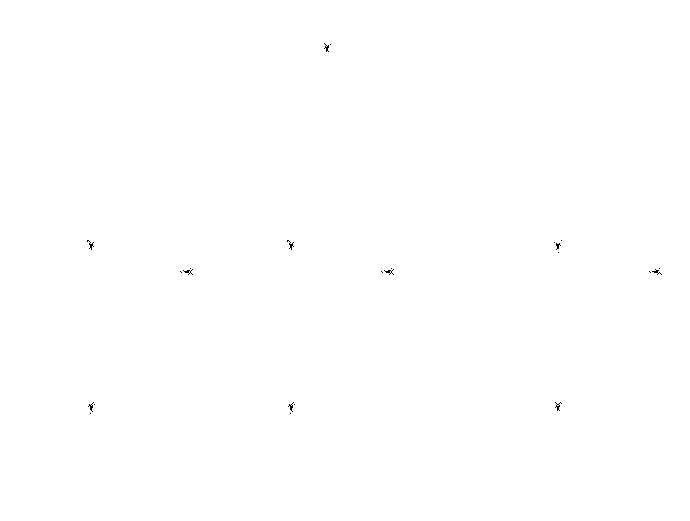
\includegraphics{fig/architecture.pdf}
        \caption{\projname algorithm architecture}
        \label{fig:architecture}
    \end{figure}

    The system starts off by instantiating metronomes with a wide range of
    tempos.  The number of metronomes is limited by the resource constraints of
    the system.  They all wait for the beat classifier to seed them with an
    initial guess at a beat, at which point they start running.  After this
    initialization phase, the metronomes keep time, each at their own tempo,
    and when the beat classifier detects a beat in the audio, it delivers a
    message to all of the metronomes stating the probability that the event it
    just saw was a beat.  The metronomes then all adjust their phase linearly
    with the probability that the beat classifier thought it was correct and
    report their current phase difference to the metronome bank controller.

    In this manner, metronomes whose tempo is different from the stream's real
    tempo will consistently report large phase errors, while those closer to
    the real tempo will report smaller phase errors.  We can then use these
    results to generate a probability distribution for the actual tempo.  After
    a period of convergence, we ``zoom in" on the possible tempos, trying
    smaller and smaller increments around the most likely tempo until we
    converge on a reasonable result.


\section{Software Implementation}

    I originally designed the algorithm in software, and even ensured that the
    software architecture looked somewhat like the hardware architecture that I
    had in my head.  The software simulation illustrates how phase-locking
    metronomes attempt to correct themselves against injected beats and return
    a phase error to the bank controller, which then figures out the most
    likely candidate for the real tempo.  Figure~\ref{fig:swscreenshot} shows a
    screenshot of the metronome bank trying to align to a seed metronome
    running at 141~BPM, which is just delivering beats.  This example converges
    very quickly because the beat classifier is ``100\% accurate."

    \begin{figure}
        \centering
        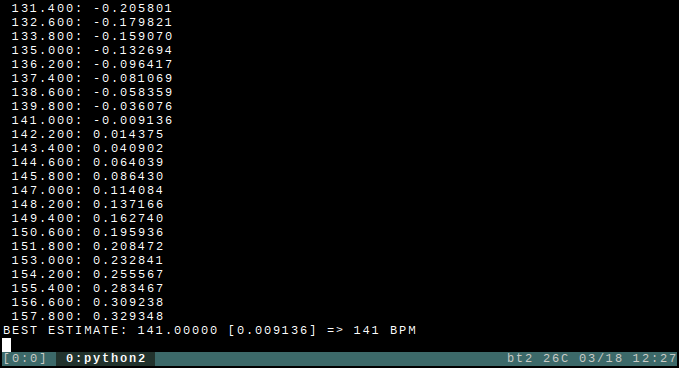
\includegraphics[scale=.5]{fig/swscreenshot.png}
        \caption{software simulation converging on seed metronome running at 141~BPM}
        \label{fig:swscreenshot}
    \end{figure}


\section{Hardware}

    For this project, I plan to use a Spartan 3-AN evaluation board that I
    already own.  I realize that this would result in my operating outside of
    the SCE-MI interface, but I'm willing to accept this risk because doing so
    gets me the extra analog hardware that I need to operate on live audio
    streams.

    The Spartan 3-AN FPGA on the eval board has 700,000 gates, 20 $18 \times
    18$ multipliers, and 360kb of BRAM.  Although it's an older FPGA without
    many of the shinier features added in later FPGAs, such as dedicated DSP
    blocks,  given the targeted small size of my design, I fully expect to stay
    in the resource constraints of the platform.  I have worked with this board
    before and already have a variety of tools that I've built for interfacing,
    so during the project time, I will be working on the actual implementation
    of the beat-tracking algorithm.

    The evaluation board has a variety of hardware, but the most important is
    the onboard ADC and pre-amplifier, which will allow me to sample audio
    directly from an input jack.  My plan is to have two input interfaces to
    the beat tracker: the first, which will be useful in simulation, will
    accept digital samples via serial.  The second will interface with the ADC,
    which is stupidly simple to control (send a pulse to initiate a conversion,
    get a response a short time later).  Both of these will provide an
    identical output interface to the beat tracker algorithm.
    Figure~\ref{fig:implementation} illustrates the overall hardware
    implementation plan.  The ADC interface and serial interface are part of
    the hardware test harness.  In hardware, one of the two is sent to the
    sample injector, which sends data to \projname.  In simulation, the sample
    injector will read from an input data file, but will present data exactly
    in the same way it does to the \projname module.  The tempo and beat output
    of \projname go to the tempo processor interface, which controls the serial
    controller and blinky LED controller (which makes the onboard LEDs blink to
    the stream).  In simulation, the tempo controller will report to
    \ttt{stdout} the tempo estimate.

    \begin{figure}
        \centering
        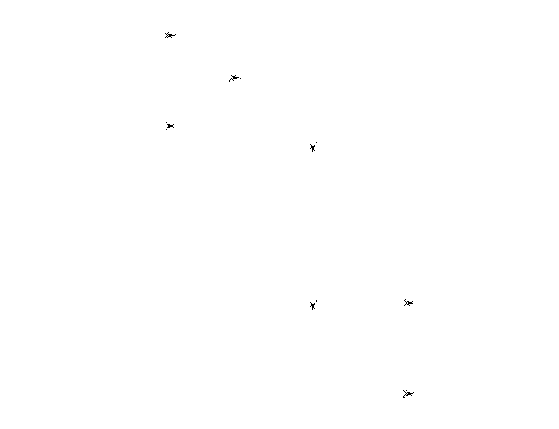
\includegraphics{fig/implementation.pdf}
        \caption{planned hardware architecture}
        \label{fig:implementation}
    \end{figure}

    I should be able to reuse a major portion of the audio pipeline's test
    harnesses, especially for developing the simulation environment.


\section{Why Implement on an FPGA?}

    Since I've already written software that can sort of do this, why should I
    go ahead and implement it on an FPGA?  In short, there are some subtle
    issues with software that I think hardware can do a lot better.

    The first is the matter of beat classification.  This overall algorithm is
    fairly robust against mediocre beat classification algorithms that
    sacrifice accuracy and precision in favor of lower computational
    complexity.  However, I'm quite convinced that with better classification
    algorithms, the system will converge to an accurate measurement
    significantly faster.

    FPGAs afford the hardware capability to perform complex tasks like FFTs and
    convolutions with very low latency, which is highly desired in a streaming
    audio platform.  I'm looking to make the convergence to an accurate tempo
    estimate as fast as possible. 

    
\section{Implementation Plan}
    
    \begin{table}[h!]
        \begin{center}
            \begin{tabular}{|rl|}
                \hline
                \textbf{week} & \textbf{tasks to be completed} \\
                \hline
                3/25 & surrounding hardware and simulation harnesses \\
                \hline
                4/1  & phase-locking metronomes and metronome bank \\
                     & controller (no field narrowing) \\
                \hline
                4/8  & first pass at a beat classifier (working demo should \\
                     & be available at this point) \\
                \hline
                4/15 & field narrowing for better convergence \\
                \hline
                4/22 & refined beat classifier \\
                \hline
                4/29 & parameter tuning \\
                \hline
                5/6  & debugging and hardware tuning \\
                \hline
                5/13  & final report \\
                \hline
            \end{tabular}
        \end{center}
        \label{tbl:sched}
    \end{table}


\end{document}
